\documentclass{article}
\usepackage[russian]{babel}

% Set page size and margins
% Replace `letterpaper' with `a4paper' for UK/EU standard size
\usepackage[letterpaper,top=2cm,bottom=2cm,left=3cm,right=3cm,marginparwidth=1.75cm]{geometry}

% Useful packages
\usepackage{amsmath}
\usepackage{graphicx}
\usepackage[colorlinks=true, allcolors=blue]{hyperref}

\title{Двумерная задача акустики на криволинейных расчётных сетках с использованием сеточно-характеристических схем первого и второго порядка точности}
\author{Семёнов, Смирнов}

\begin{document}
\maketitle

\section{Теория}

\subsection{Численный метод}
Хотим решить двумерную акустическую задачу. В общем виде уравнение 2D акустики выглядит следующим образом:
\begin{equation}
    \overrightarrow{q_t} + A_1\overrightarrow{q_x} + A_2\overrightarrow{q_y} = \overrightarrow{f}
\end{equation}
где\\
\overrightarrow{q}=
\begin{pmatrix}
v_x&v_y&p\\
\end{pmatrix}\\
\\
$A_1$=
\begin{pmatrix}
0&0&1/\rho\\
0&0&0\\
\rho c^2&0&0\\
\end{pmatrix};
$A_2$=
\begin{pmatrix}
0&0&0\\
0&0&1/\rho\\
0&\rho c^2&0\\
\end{pmatrix}\\
Для решения будем использовать сеточно-характеристический метод. Который состоит в том, что мы разбиваем исходное уравнение сперва на два однородных (по $x$ и по $y$), а затем решаем $\overrightarrow{q_t}=\overrightarrow{f}$.\\
Первые два шага для $x$ и $y$ аналогичны, поэтому для сокращения будем писать индекс $i$ вместо них.\\
\textbf{Шаг1.} Рассмотрим одномерное уравнение:
\begin{equation}
    \overrightarrow{q_t} + A_i\overrightarrow{q_i} = \overrightarrow{0}
\end{equation}
В таком случае можем представить матрицу в виде:
\begin{equation}
    A_i = \Omega^{-1}_i\Lambda\Omega_i
\end{equation}
Эти матрицы равны:
$\Omega_x$=
\begin{pmatrix}
0&1&0&\\
-\rho c/2&0&1/2\\
\rho c/2&0&1/2\\
\end{pmatrix};
$\Omega^{-1}_x$=
\begin{pmatrix}
0&-\frac{1}{\rho c}&\frac{1}{\rho c}&\\
1&0&0\\
0&1&1\\
\end{pmatrix};
$\Omega_y$=
\begin{pmatrix}
1&0&0&\\
0&-\rho c/2&1/2\\
0&\rho c/2&1/2\\
\end{pmatrix};
$\Omega^{-1}_y$=
\begin{pmatrix}
1&0&0&\\
0&-\frac{1}{\rho c}&-\frac{1}{\rho c}\\
0&1&1\\
\end{pmatrix};
$\Lambda$=
\begin{pmatrix}
0&0&0&\\
0&-c&0\\
0&0&c\\
\end{pmatrix}\\
Риманов инвариант:
\begin{equation}
    \overrightarrow{\omega}=\Omega_i\overrightarrow{q}
\end{equation}
\textbf{Шаг2.} Умножая (2) на $\Omega_i$ получим:
\begin{equation}
    \overrightarrow{\omega_t} + \Lambda\overrightarrow{\omega_i} = \overrightarrow{0}
\end{equation}
\textbf{Шаг3.}Решим уравнение (5) используя характеристическое свойство:
\begin{equation}
    \omega_j(t+dt,x)=\omega_j(t,x-\lambda_j dt)
\end{equation}
Это нам необходимо чтобы проводить интерполяцию. Приступим к ней:\\
дифференцируя по $i$(либо $x$ либо $y$)гладкую (предполагаем) функцию $\overrightarrow{q}$
\begin{equation}
(\overrightarrow{q_i})_t + A_i(\overrightarrow{q_i})_i=\overrightarrow{0}
\end{equation}
Примем $\overrightarrow{q_i}$ за новую переменную и введем ещё один Риманов инвариант:
\begin{equation}
    \overrightarrow{w}=\Omega_i\overrightarrow{q_i}
\end{equation}
Т.о., после процедуры интерполяции, мы будем знать $\omega$ и $w$ для следующего шага $t+dt$ и перейдя обратно к $\overrightarrow{q_i}$, $\overrightarrow{q}$ через обратные матрицы $\Omega_i$.\\
Для корректности проведения данной процедуры на следующих шагах нам надо также знать значения вторых производных $\overrightarrow{q_{xy}}$ и $\overrightarrow{q_k}$ ($k\neq i$). В таком случае получим систему уравнений:
\begin{equation}
    \begin{cases}
    (\overrightarrow{q_k})_t + A_i(\overrightarrow{q_k})_i = \overrightarrow{0}
    \\
    (\overrightarrow{q_{xy}})_t + A_i(\overrightarrow{q_{xy}})_i = \overrightarrow{0}
    \end{cases}
\end{equation}

\subsection{Криволинейная сетка}
Наша задача $--$ перейти в исходном уравнении в полярные координаты $(r, \varphi)$ и выяснить как изменятся матрицы $A_1$, $A_2$ на $\widetilde{A_1}$, $\widetilde{A_2}$.\\
Тогда известные нам производные преобразуются в как:
\begin{equation}
    \frac{\partial p}{\partial x}=\frac{1}{\cos{\varphi}}\frac{\partial p}{\partial r}-\frac{1}{r}\cot{\varphi}\frac{\partial p}{\partial \varphi}
\end{equation}
\begin{equation}
    \frac{\partial p}{\partial y}=\frac{1}{\sin{\varphi}}\frac{\partial p}{\partial r}+\frac{1}{r}\tan{\varphi}\frac{\partial p}{\partial \varphi}
\end{equation}
\begin{equation}
    \frac{\partial v_x}{\partial x}=\frac{\partial v_r}{\partial r}+\cot{\varphi}\frac{\partial v_{\varphi}}{\partial \varphi}
\end{equation}
\begin{equation}
    \frac{\partial v_y}{\partial y}=\frac{\partial v_r}{\partial r}-\tan{\varphi}\frac{\partial v_{\varphi}}{\partial \varphi}
\end{equation}
Следовательно, система уравнений $(1)$ преобразуется в:
\begin{equation}
    \overrightarrow{q_t} + \widetilde{A_1}\overrightarrow{q_r} + \widetilde{A_2}\overrightarrow{q_{\varphi}} = \overrightarrow{f}
\end{equation}
где\\
\overrightarrow{q}=
\begin{pmatrix}
v_r&v_{\varphi}&p\\
\end{pmatrix}\\
\\
$\widetilde{A_1}$=
\begin{pmatrix}
0&0&\frac{1}{\rho \cos{\varphi}}\\
0&0&\frac{1}{\rho \sin{\varphi}}\\
2\rho c^2&0&0\\
\end{pmatrix};
$\widetilde{A_2}$=
\begin{pmatrix}
0&0&-\frac{1}{r\rho}\cot{\varphi}\\
0&0&\frac{1}{r\rho}\tan{\varphi}\\
0&2\rho c^2\cot{2\varphi}&0\\
\end{pmatrix}\\
По сеточно-характеристическому методу составим матрицы:
\section{Реализация на Python}
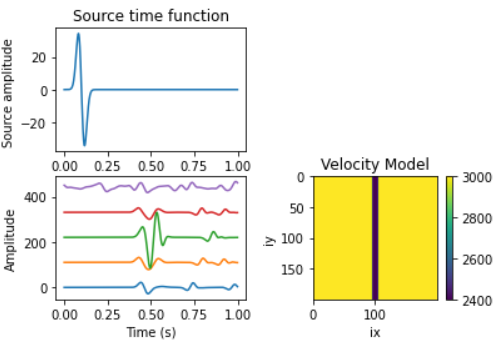
\includegraphics[width=1\linewidth]{111}
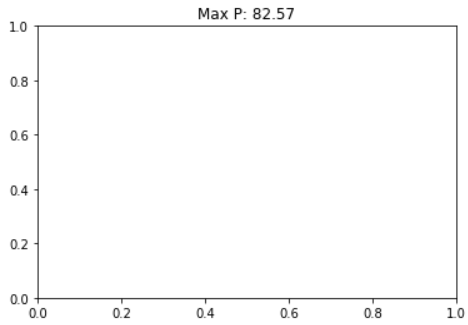
\includegraphics[width=1\linewidth]{112}
\section{Выводы}


\end{document}